\de{ĐỀ THI ÔN TẬP HỌC KỲ I NĂM HỌC 2022-2023}{THPT Đống Đa - Hà Nội}


\begin{center}
	\textbf{PHẦN 1 - TRẮC NGHIỆM}
\end{center}
\Opensolutionfile{ans}[ans/ans]

\begin{ex}%[0D4Y1-2]%[Dự án đề kiểm tra HKI NH22-23- Lương Như Quỳnh]%[Trường THPT Đống Đa]
Cho tam thức $f(x)=a x^2+b x+c \quad(a \neq 0)$, $\Delta=b^2-4 a c$. Ta có $f(x) \leq 0$ với $\forall x \in \mathbb{R}$ khi và chi khi
\choice
{$\heva{&a>0\\ &\Delta \leq 0}$}
{\True $\heva{&a<0\\ &\Delta \leq 0}$}
{$\heva{&a<0\\ &\Delta<0}$}
{$\heva{&a<0\\ &\Delta \geq 0}$}
\loigiai{
Ta có $f(x) \leq 0$ với $\forall x \in \mathbb{R}$ khi và chi khi $\heva{&a<0\\ &\Delta \leq 0.}$
}
\end{ex}

\begin{ex}%[0D3B2-2]%[Dự án đề kiểm tra HKI NH22-23- Lương Như Quỳnh]%[Trường THPT Đống Đa]
Cho hàm số $y=x^2-2x+4$ có đồ thị $(P)$. Tìm mệnh đề {\bf sai}.
\choice
{$\max y=7$, $\forall x \in[0;3]$}
{\True $\min y=4$, $\forall x \in[0;3]$}
{$(P)$ có trục đối xứng $x=1$}
{$(P)$ có đỉnh $I(1;3)$}
\loigiai{
Parabol $(P)$  
\begin{itemize}
			\item Có đỉnh $I(1;3)$;
			\item Có trục đối xứng là đường thẳng $x=1$;
			\item Bề lõm quay lên trên vì $a=1>0$;
			\item Đi qua $(0;4)$, $(3;7)$.
			\item Bảng biến thiên trên $[0;3]$
		\begin{center}
		
\begin{tikzpicture}[>=stealth]
		\tkzTabInit[nocadre=false,lgt=1,espcl=2.5,deltacl=0.5]{$x$/.7,$y$/2}
		{$0$ , $1$ , $3$}
		\tkzTabVar{+/$4$ , -/$3$ , +/$7$}
		\end{tikzpicture}
		\end{center}
			Dựa vào bảng biến thiên nhận thấy $\max y=7$, $\forall x \in[0;3]$ và $\min y=3$, $\forall x \in[0;3]$.
\end{itemize}
}
\end{ex} 

\begin{ex}%[0D4B3-2]%[Dự án đề kiểm tra HKI NH22-23- Lương Như Quỳnh]%[Trường THPT Đống Đa]
Khi giải phương trình $\sqrt{x^2+3 x}+1=3 x$ $\quad(1)$ ta tiến hành theo các bước sau:\\
Bước 1: Bình phương hai vế của phương trình $(1)$ ta được $x^2+3 x=(3 x-1)^2 \quad (2)$.\\
Bước 2: Khai triển và rút gọn $(2)$ ta được $8 x^2-9 x+1=0 \Leftrightarrow \hoac{&x=1 \\ &x=\dfrac{1}{8}.}$\\
Bước 3: Khi $x=1$, ta có $x^2+3 x>0$. Khi $x=\dfrac{1}{8}$, ta có $x^2+3 x>0$.\\
Vậy tập nghiệm của phương trình là $S=\left\{1;\dfrac{1}{8}\right\}$.\\
Cách giải trên đúng hay sai? Nếu sai thì sai ở bước nào?
\choice
{\True Sai ở bước 3}
{Sai ở bước 1}
{Đúng}
{Sai ở bước 2}
\loigiai{
Cách giải trên sai ở bước $3$. Sửa lại như sau.\\
Bước 3: Khi $x=1$, ta có $3x-1>0$. Khi $x=\dfrac{1}{8}$, ta có $3x-1<0$.\\
Vậy tập nghiệm của phương trình là $S=\left\{1\right\}$.\\
}
\end{ex} 

\begin{ex}%[0D4B2-1]%[Dự án đề kiểm tra HKI NH22-23- Lương Như Quỳnh]%[Trường THPT Đống Đa]
Tìm tập xác định của hàm số $y=\sqrt{2x^2-5x+2}$.
\choice
{$[2 ;+\infty)$}
{$\left(-\infty ; \dfrac{1}{2}\right]$}
{$\left[\dfrac{1}{2} ; 2\right]$}
{\True $\left(-\infty ; \dfrac{1}{2}\right] \cup[2 ;+\infty)$}
\loigiai{
Hàm số đã cho xác định khi và chỉ khi $ 2x^2-5x+2\geq 0\Leftrightarrow \hoac{&x\leq \dfrac{1}{2}\\&x\geq 2.} $\\
Vậy tập xác định của hàm số đã cho là $ \mathscr{D}=\left(-\infty ; \dfrac{1}{2}\right] \cup[2 ;+\infty)$.
}
\end{ex} 

\begin{ex}%[0D3B2-3]%[Dự án đề kiểm tra HKI NH22-23- Lương Như Quỳnh]%[Trường THPT Đống Đa]
\immini{
Hàm số nào có đồ thị như hình vẽ bên?
\choice
{$y=x^2-4 x-3$}
{$y=-x^2-4 x-3$}
{\True $y=-x^2+4 x-3$}
{$y=-2 x^2-x-3$}}{
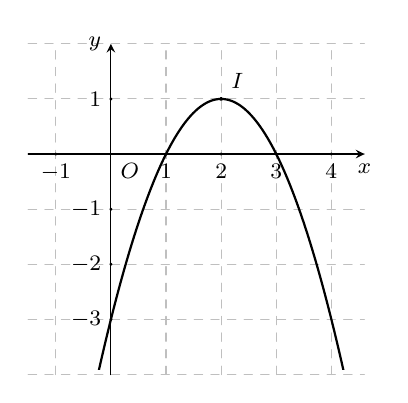
\begin{tikzpicture}[>=stealth,line join=round,line cap=round,font=\footnotesize,scale=.7]
	\def\a{-1}
	\def\b{4}
	\def\c{-3}
	\def\xmin{-1.5} \def\xmax{4.6}
	\def\ymin{-4} \def\ymax{2} 
	\draw[color=gray!50,dashed] (\xmin,\ymin) grid (\xmax,\ymax); 
	\draw[->] (\xmin,0)--(\xmax,0) node [below]{$x$};
	\draw[->] (0,\ymin)--(0,\ymax) node [left]{$y$};
	\node at (0,0) [below right]{$O$};
	\foreach \x in{-1,1,2,3,4}\draw[fill=black] (\x,0) circle (.5pt) node[below]{\footnotesize $\x$};
	\foreach \y in{-3,-2,-1,1}\draw[fill=black] (0,\y)circle (.5pt) node[left]{\footnotesize $\y$};	
	\clip (\xmin+0.1,\ymin+0.1) rectangle (\xmax-0.1,\ymax-0.1);
	\pgfmathsetmacro\xdinh{-(\b)/2*(\a)}
	\pgfmathsetmacro\ydinh{(4*(\a)*(\c)-(\b)^2)/(4*(\a))}		
\draw[thick,samples=150,smooth,domain=\xmin:\xmax] plot(\x,{\a*(\x)^2+(\b)*\x+(\c)})
	(2,1)circle (.5pt) node[above right]{$I$}
	;
			\end{tikzpicture}
}
\loigiai{
Dựa vào đồ thị ta thấy Parabol có đỉnh $I(2;1)$ nên các hàm số $y=-2x^2-x-3$, $y=x^2-4x-3$, $y=-x^2-4x-3$ không thỏa mãn.\\
Vậy hàm số $y=-x^2+4x-3$ có đồ thị như hình vẽ.
}
\end{ex} 

\begin{ex}%[0H2B2-4]%[Dự án đề kiểm tra HKI NH22-23- Lương Như Quỳnh]%[Trường THPT Đống Đa]
Cho $\triangle ABC$, gọi điểm $M$ thỏa $\overrightarrow{MA}+\overrightarrow{BC}-\overrightarrow{BM}-\overrightarrow{AB}=\overrightarrow{BA}$. Mệnh đề nào sau đây đúng?
\choice
{$M$ là trọng tâm $\triangle ABC$}
{$M$ là trung điểm $AB$}
{\True $M$ là trung điểm $CA$}
{$M$ là trung điểm $BC$}
\loigiai{
Ta có 
\allowdisplaybreaks
\begin{eqnarray*}
 && \overrightarrow{MA}+\overrightarrow{BC}-\overrightarrow{BM}-\overrightarrow{AB}=\overrightarrow{BA} \\ 
  &\Leftrightarrow& \overrightarrow{MA}+\overrightarrow{MC}=\overrightarrow{AB}+\overrightarrow{BA}\\ 
  &\Leftrightarrow& \overrightarrow{MA}+\overrightarrow{MC}=\overrightarrow{0}.
\end{eqnarray*}
Suy ra $M$ là trung điểm $CA$.
}
\end{ex} 

\begin{ex}%[0D3B2-2]%[Dự án đề kiểm tra HKI NH22-23- Lương Như Quỳnh]%[Trường THPT Đống Đa]
Bảng biến thiên sau là của hàm số nào?
		\begin{center}
		
\begin{tikzpicture}[>=stealth]
	\tkzTabInit[nocadre=false,lgt=1,espcl=2.5,deltacl=0.5]{$x$/.7,$y$/2}
		{$-\infty$ , $1$ , $+\infty$}
		\tkzTabVar{+/$+\infty$ , -/$2$ , +/$+\infty$}
		\end{tikzpicture}
		\end{center}
\choice
{$y=x^2-2x+2$}
{$y=-3x^2+6x-1$}
{$y=x^2+2x-1$}
{\True $y=2x^2-4x+4$}
\loigiai{
Bảng biến thiên đã cho là của hàm số bậc hai, có đồ thị là  Parabol $(P)$.
\begin{itemize}
			\item Bề lõm $(P)$ quay lên trên suy ra $a>0$, nên hàm số $y=-3x^2+6x-1$ không thỏa mãn;
			\item $(P)$ có đỉnh $I(1;2)$ nên các hàm số $y=x^2-2x+2$, $y=x^2+2x-1$ không thỏa mãn.
\end{itemize}
Vậy hàm số $y=2x^2-4x+4$ có bảng biến thiên đã cho.
}
\end{ex}

\begin{ex}%[0D4B1-2]%[Dự án đề kiểm tra HKI NH22-23- Lương Như Quỳnh]%[Trường THPT Đống Đa]
Tam thức nào dưới đây luôn dương với mọi giá trị của $x$?
\choice
{$-x^2+2x+10$}
{$x^2-2x-10$}
{\True $x^2-2x+10$}
{$x^2-10x+2$}
\loigiai{
Xét tam thức $x^2-2x+10$ ta có $ \heva{&a=1>0\\&\Delta=-9<0} $ suy ra $x^2-2x+10>0$, $\forall x\in \mathbb{R}$.
}
\end{ex}

\begin{ex}%[0H2B4-5]%[Dự án đề kiểm tra HKI NH22-23- Lương Như Quỳnh]%[Trường THPT Đống Đa]
Cho ba điểm $A$, $B$, $C$ phân biệt. Tập hợp những điểm $M$ mà $\overrightarrow{CM} \cdot \overrightarrow{CB}=\overrightarrow{CA} \cdot \overrightarrow{CB}$ là
\choice
{\True Đường thẳng đi qua $A$ và vuông góc với $BC$}
{Đường thẳng đi qua $B$ và vuông góc với $AC$}
{Đường tròn đường kính $AB$}
{Đường thẳng đi qua $C$ và vuông góc với $AB$}
\loigiai{
Ta có 
\allowdisplaybreaks
\begin{eqnarray*}
 && \overrightarrow{CM} \cdot \overrightarrow{CB}=\overrightarrow{CA} \cdot \overrightarrow{CB} \\ 
  &\Leftrightarrow& \overrightarrow{CB}\left(\overrightarrow{CM}-\overrightarrow{CA}\right)=0\\ 
  &\Leftrightarrow& \overrightarrow{CB}\cdot\overrightarrow{AM}=0.
\end{eqnarray*}
Suy ra tập hợp những điểm $M$ là đường thẳng đi qua $A$ và vuông góc với $BC$.
}
\end{ex}

\begin{ex}%[0D4B2-1]%[Dự án đề kiểm tra HKI NH22-23- Lương Như Quỳnh]%[Trường THPT Đống Đa]
Cho tam thức bậc hai $f(x)=-x^2-4x+5$. Tìm tất cả giá trị của $x$ để $f(x)\geq 0$.
\choice
{$x \in(-\infty ;-1] \cup[5;+\infty)$}
{$x \in(-5;1)$}
{$x \in[-1;5]$}
{\True $x \in[-5;1]$}
\loigiai{
Ta có $f(x)\geq 0 \Leftrightarrow -x^2-4x+5\geq 0\Leftrightarrow -5\leq x\leq 1$.
}
\end{ex}

\begin{ex}%[0T3B1-2]%[Dự án đề kiểm tra HKI NH22-23- Lương Như Quỳnh]%[Trường THPT Đống Đa]
Cho ba điểm $A$, $B$, $C$ phân biệt và thẳng hàng. Mệnh đề nào sau đây đúng?
\choice
{$\overrightarrow{AB}$ và $\overrightarrow{A C}$ ngược hướng}
{$\overrightarrow{CA}$ và $\overrightarrow{CB}$ cùng hướng}
{\True $\overrightarrow{BA}$ và $\overrightarrow{BC}$ cùng phương}
{$\overrightarrow{AB}=\overrightarrow{BC}$}
\loigiai{
Với ba điểm $A$, $B$, $C$ phân biệt và thẳng hàng, ta có $\overrightarrow{BA}$ và $\overrightarrow{BC}$ cùng phương.
}
\end{ex}

\begin{ex}%[0D3B2-3]%[Dự án đề kiểm tra HKI NH22-23- Lương Như Quỳnh]%[Trường THPT Đống Đa]
\immini{Cho hàm số $ y=f(x)=ax^2+bx+c $ có đồ thị như hình vẽ bên. Đặt $\Delta=b^2-4ac$, tìm dấu của $a$ và $\Delta$.
\choice
{$a<0$, $\Delta>0$}
{$a<0$, $\Delta=0$}
{\True $a>0$, $\Delta>0$}
{$a>0$, $\Delta=0$}}{
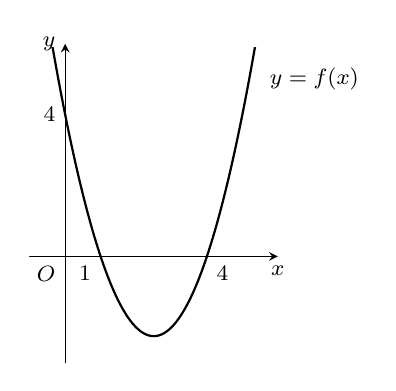
\begin{tikzpicture}[>=stealth,line join=round,line cap=round,font=\footnotesize,scale=.45]
					\def\a{1}
					\def\b{-5}
					\def\c{4}
					\def\xmin{-1} \def\xmax{6}
	\def\ymin{-3} \def\ymax{6}  
	\draw[->] (\xmin,0)--(\xmax,0) node [below]{$x$};
	\draw[->] (0,\ymin)--(0,\ymax) node [left]{$y$};
	\node at (0,0) [below left]{$O$};
					\fill 
					(1,0)circle(1pt)node[below left]{$1$}
					(0,4)circle(1pt)node[left]{$4$}
					(4,0)circle(1pt)node[below right]{$4$}
					(5.5,5) node[right]{$y=f(x)$}
					;
	\clip (\xmin+0.1,\ymin+0.1) rectangle (\xmax-0.1,\ymax-0.1);		
\draw[thick,samples=150,smooth,domain=\xmin:\xmax] plot(\x,{\a*(\x)^2+(\b)*\x+(\c)});
			\end{tikzpicture}
}
\loigiai{
Dựa vào đồ thị ta thấy 
\begin{itemize}
			\item Parabol có bề lõm quay lên trên suy ra $a>0$.
			\item Parabol cắt trục hoành tại hai điểm phân biệt suy ra $\Delta>0$.
\end{itemize}
}
\end{ex}

\begin{ex}%[0H2B3-5]%[Dự án đề kiểm tra HKI NH22-23- Lương Như Quỳnh]%[Trường THPT Đống Đa]
Cho hình chữ nhật $ABCD$. Gọi $I$, $K$ lần lượt là trung điểm của $BC$ và $CD$. Chọn đẳng thức đúng.
\choice
{$\overrightarrow{AI}+\overrightarrow{AK}=\overrightarrow{IK}$}
{$\overrightarrow{AI}+\overrightarrow{AK}=2 \overrightarrow{AC}$}
{$\overrightarrow{AI}+\overrightarrow{AK}=\overrightarrow{AB}+\overrightarrow{AD}$}
{\True $\overrightarrow{AI}+\overrightarrow{AK}=\dfrac{3}{2} \overrightarrow{AC}$}
\loigiai{\immini{
Ta có $I$, $K$ lần lượt là trung điểm của $BC$ và $CD$ nên
\[
\heva{&\overrightarrow{AI}=\dfrac{1}{2}\left(\overrightarrow{AB}+\overrightarrow{AC}\right)\\&\overrightarrow{AK}=\dfrac{1}{2}\left(\overrightarrow{AC}+\overrightarrow{AD}\right).}
\]
Suy ra 
\allowdisplaybreaks
\begin{eqnarray*}
 && \overrightarrow{AI}+\overrightarrow{AK} \\ 
  &=&  \dfrac{1}{2}\left(2\overrightarrow{AC}+\overrightarrow{AB}+\overrightarrow{AD}\right)\\ 
  &=&  \dfrac{1}{2}\left(2\overrightarrow{AC}+\overrightarrow{AC}\right)\\ 
  &=& \dfrac{3}{2}\overrightarrow{AC}.
\end{eqnarray*}}{
\begin{tikzpicture}
\path (0,0) coordinate (A)
	($(90:2)$)coordinate(B)
	($(0:5)$)coordinate(D)
	($ (B)+(D)-(A) $)coordinate (C)
	($ (B)!.5!(C) $)coordinate (I)
	($ (D)!.5!(C) $)coordinate (K)
	;
	\draw (A)--(C) (A)--(B)--(C)--(D)--cycle (A)--(I)--(K)--cycle;
	\foreach \t/\g in {A/180,B/180,D/0,C/0,I/90,K/0}{
	\draw[fill=black] (\t) circle (1pt) node[shift={(\g:7pt)},font=\scriptsize]{$ \t $};
		}	
	\end{tikzpicture}
}
}
\end{ex}


%%%% Câu 14
\begin{ex}%[0H2Y2-1]%[Dự án đề kiểm tra HKI NH22-23 - Thành Đức Trung]%[THPT Đống Đa - Hà Nội]
Cho ba điểm phân biệt $A$, $B$, $C$. Trong các khẳng định sau, khẳng định nào \textbf{sai}?
\choice
{$\overrightarrow{CA}+\overrightarrow{BC}=\overrightarrow{BA}$}
{\True $\overrightarrow{CB}+\overrightarrow{AC}=\overrightarrow{BA}$}
{$\overrightarrow{AC}+\overrightarrow{CB}=\overrightarrow{AB}$}
{$\overrightarrow{AB}+\overrightarrow{BC}=\overrightarrow{AC}$}
\loigiai
{Theo quy tắc ba điểm, ta có $\overrightarrow{CB}+\overrightarrow{AC}=\overrightarrow{AB}$ nên khẳng định sai là $\overrightarrow{CB}+\overrightarrow{AC}=\overrightarrow{BA}$.
}
\end{ex}

%%%% Câu 15
\begin{ex}%[0H2B3-4] %[Dự án đề kiểm tra HKI NH22-23 - Thành Đức Trung]%[THPT Đống Đa - Hà Nội]
Biết rằng hai véc-tơ $\overrightarrow{a}$ và $\overrightarrow{b}$ không cùng phương nhưng hai véc-tơ $3\overrightarrow{a}-2\overrightarrow{b}$ và $(x+1)\overrightarrow{a}+4\overrightarrow{b}$ cùng phương. Khi đó giá trị của $x$ là
\choice
{$7$}
{$5$}
{\True $-7$}
{$6$}
\loigiai
{Do $3\overrightarrow{a}-2\overrightarrow{b}$ và $(x+1)\overrightarrow{a}+4\overrightarrow{b}$ cùng phương nên $3\overrightarrow{a}-2\overrightarrow{b}=k[(x+1)\overrightarrow{a}+4\overrightarrow{b}]$ (với $k\ne0$).\\
Suy ra $[3-k(x+1)]\overrightarrow{a}+(-2-4k)\overrightarrow{b}=\overrightarrow{0}$ \quad (1).\\
Do $\overrightarrow{a}$ không cùng phương với $\overrightarrow{b}$ nên từ (1) suy ra $\heva{&3-k(x+1)=0\\&-2-4k=0}\Leftrightarrow\heva{&x=-7\\&k=-\dfrac{1}{2}.}$
}
\end{ex}

%%%% Câu 16
\begin{ex}%[0D4K3-3]%[Dự án đề kiểm tra HKI NH22-23 - Thành Đức Trung]%[THPT Đống Đa - Hà Nội]
Tìm $m$ để phương trình $\sqrt{2x^2-2x-2m}=x-2$ có nghiệm.
\choice
{$m>2$}
{\True $m\ge2$}
{$m\le1$}
{$m\in(1;+\infty)$}
\loigiai
{
Ta có $\sqrt{2x^2-2x-2m}=x-2 \Leftrightarrow \heva{ & x\geq2 \\ & 2x^2-2x-2m=\left(x-2\right)^2} \Leftrightarrow \heva{ & x\geq2 \\ & 2m=x^2+2x-4. \quad (1)}$ \\
Xét hàm số $f(x)=x^2+2x-4$. \\
Bảng biến thiên của $f(x)$ như sau
\begin{center}

\begin{tikzpicture}[scale=1, >=stealth]
\tkzTabInit[nocadre=false, lgt=1.2, espcl=3.5, deltacl=0.6]{$x$/0.6, $f(x)$/2}{$-\infty$, $-1$, $+\infty$}
\tkzTabVar{+/$+\infty$, -/$-5$, +/$+\infty$}
\tkzTabVal{2}{3}{0.5}{$2$}{$4$}
\end{tikzpicture}
\end{center}
Phương trình đã cho có nghiệm khi phương trình $(1)$ có nghiệm trên $[2;+\infty)$. \\
Từ bảng biến thiên ta có $2m\geq4 \Leftrightarrow m\geq2$.
}
\end{ex}

%%%% Câu 17
\begin{ex}%[0H2B2-5]%[Dự án đề kiểm tra HKI NH22-23 - Thành Đức Trung]%[THPT Đống Đa - Hà Nội]
Cho hình vuông $ABCD$ có cạnh là $a$. Gọi $O$ là giao điểm của hai đường chéo. Tính $\left|\overrightarrow{OA}-\overrightarrow{CB}\right|$.
\choice
{\True $\dfrac{a\sqrt{2}}{2}$}
{$a\sqrt{3}$}
{$\dfrac{a\sqrt{3}}{2}$}
{$a\sqrt{2}$}
\loigiai
{\immini{Do $ABCD$ là hình vuông nên ta có $\overrightarrow{OA}-\overrightarrow{CB}=\overrightarrow{CO}-\overrightarrow{CB}=\overrightarrow{BO}$.\\
Suy ra $\left|\overrightarrow{OA}-\overrightarrow{CB}\right|=\left|\overrightarrow{BO}\right|=BO=\dfrac{a\sqrt{2}}{2}$.}
{\begin{tikzpicture}[scale=1, font=\footnotesize,>=stealth]%<DTools>
\def\canhBA{3};\def\canhCB{3};\def\canhAD{3};
%Định nghĩa điểm.
\coordinate (B) at (0,0);
\coordinate (A) at (90:\canhBA);
\coordinate (C) at (0:\canhCB);
\coordinate (D) at (3,3);
\coordinate (O) at (1.5,1.5);
%Vẽ tam giác vuông ABC.
\draw (B)--(A)--(C)--(D)--cycle;
\draw (B)--(C) (A)--(D);
\draw pic[draw, angle radius=3mm, angle eccentricity=1.5]{right angle = A--B--C};
%Hiển thị các điểm.
\foreach \x/\y in {B/180,A/90,C/0,D/90,O/-90}{\fill (\x)circle (1pt) ($(\x)+(\y:0.3cm)$) node{$\x$};}
\end{tikzpicture}}
}
\end{ex}

%%%% Câu 18
\begin{ex}%[0H2B4-1]%[Dự án đề kiểm tra HKI NH22-23 - Thành Đức Trung]%[THPT Đống Đa - Hà Nội]
Cho tam giác đều $ABC$ có cạnh bằng $a$. Tính tích vô hướng $\overrightarrow{AB}\cdot \overrightarrow{AC}$.
\choice
{$2a^2$}
{$-\dfrac{a^2\sqrt{3}}{2}$}
{\True $\dfrac{a^2}{2}$}
{$-\dfrac{a^2}{2}$}
\loigiai
{Ta có $\overrightarrow{AB}\cdot \overrightarrow{AC}=|\overrightarrow{AB}|\cdot| \overrightarrow{AC}|\cos(\overrightarrow{AB}, \overrightarrow{AC})=a\cdot a \cos60^\circ = \dfrac{a^2}{2}.$
}
\end{ex}

%%%% Câu 19
\begin{ex}%[0D3B2-2]%[Dự án đề kiểm tra HKI NH22-23 - Thành Đức Trung]%[THPT Đống Đa - Hà Nội]
Cho hàm số $y = -x^2+4x+1$. Khẳng định nào sau đây là \textbf{sai}?
\choice
{Hàm số nghịch biến trên khoảng $(2;+\infty)$ và đồng biến trên khoảng $(-\infty; 2)$}
{\True Trên khoảng $(-\infty; 1)$ hàm số đồng biến}
{Hàm số nghịch biến trên khoảng $(4; +\infty)$ và đồng biến trên khoảng $(-\infty; 4)$}
{Trên khoảng $(3;+\infty)$ hàm số nghịch biến}
\loigiai
{Ta có $-\dfrac{b}{2a}=2; -\dfrac{\Delta}{4a}=5.$\\
Vì $a =-1<0$ nên hàm số nghịch biến trên khoảng $(2;+\infty)$ và đồng biến trên khoảng $(-\infty; 2)$.
}
\end{ex}

%%%% Câu 20
\begin{ex}%[0D3B2-1]%[Dự án đề kiểm tra HKI NH22-23 - Thành Đức Trung]%[THPT Đống Đa - Hà Nội]
Tìm $m$ để phương trình $-x^2+2(m-1)x+m-3=0$ có hai nghiệm phân biệt
\choice
{$(-1;2)$}
{$[-1;2]$}
{\True $(-\infty;-1)\cup(2;+\infty)$}
{$(-\infty;-1]\cup[2;+\infty)$}
\loigiai
{Phương trình đã cho có hai nghiệm phân biệt\\
$\Leftrightarrow\heva{&a\ne0\\&\Delta'>0}\Leftrightarrow\heva{&-1\ne 0\\&(m-1)^2+m-3>0}\Leftrightarrow m^2-m-2>0\Leftrightarrow \hoac{&m<-1\\&m>2.}$\\
Vậy $m\in(-\infty;-1)\cup(2;+\infty)$ thì phương trình đã cho có hai nghiệm.
}
\end{ex}

%%%% Câu 21
\begin{ex}%[0D4K2-1]%[Dự án đề kiểm tra HKI NH22-23 - Thành Đức Trung]%[THPT Đống Đa - Hà Nội]
Tìm tập hợp các giá trị của tham số $m$ để hàm số $y = \sqrt{(m+10)x^2-2(m-2)x+1}$ có tập xác định là $\mathscr{D}=\mathbb{R}$.
\choice
{$(-1;6)$}
{$[-1;6]$}
{$(-\infty;-1)\cup (6;+\infty)$}
{$\mathbb{R}$}
\loigiai
{Điều kiện xác định $(m+10)x^2-2(m-2)x+1\geq 0$.\\
\underline{TH1:} Với $m+10 =0 \Leftrightarrow m =-10$, khi đó điều kiện xác định trở thành $24x+1\geq 0\Leftrightarrow x \geq -\dfrac{1}{24}$.\\
Suy ra $m =-10$ không thỏa mãn yêu cầu bài toán.\\
\underline{TH2:} Với $m+10 \ne0 \Leftrightarrow m \ne-10$, khi đó để hàm số có tập xác định $\mathscr{D} =\mathbb{R}$
\begin{align*}
&\Leftrightarrow (m+10)x^2-2(m-2)x+1\geq 0\, \forall x \in \mathbb{R}\\& \Leftrightarrow \heva{&m+10>0\\&4(m-2)^2-4(m+10) \leq 0}\\& \Leftrightarrow \heva{&m>-10\\&m^2-5m-6 \leq 0}\\& \Leftrightarrow \heva{&m>-10\\&-1\leq m\leq 6}\\&\Leftrightarrow -1\leq m\leq 6.
\end{align*}
Vậy $m\in [-1;6]$ thì hàm số đã cho có tập xác định $\mathscr{D}=\mathbb{R}$.
}
\end{ex}

%%%% Câu 22
\begin{ex}%[0D4B3-2]%[Dự án đề kiểm tra HKI NH22-23 - Thành Đức Trung]%[THPT Đống Đa - Hà Nội]
Tổng các nghiệm (nếu có) của phương trình $\sqrt{2x-1} = x-2$ bằng
\choice
{$6$}
{$2$}
{\True $5$}
{$1$}
\loigiai
{
Ta có 
\[\sqrt{2x-1} = x-2 \Leftrightarrow \heva{&x-2\ge 2\\&2x-1=(x-2)^2} \Leftrightarrow \heva{&x\ge 2\\&x^2 - 6x + 5 = 0} \Leftrightarrow \heva{&x\ge 2\\&\hoac{&x=1\\&x=5}} \Leftrightarrow x=5.\]
}
\end{ex}

%%%% Câu 23
\begin{ex}%[0H2B1-3]%[Dự án đề kiểm tra HKI NH22-23 - Thành Đức Trung]%[THPT Đống Đa - Hà Nội]
Cho hình bình hành $ABCD$. Gọi $O$ là giao điểm của hai đường chéo $AC$ và $BD$. Điểm $M$ thỏa mãn đẳng thức $\overrightarrow{AB} + \overrightarrow{AC} + \overrightarrow{AD} = 4\overrightarrow{AM}$. Khi đó điểm $M$ trùng với điểm
\choice
{$I$ là trung điểm đoạn $OC$}
{$I$ là trung điểm đoạn $OA$}
{$C$}
{\True $O$}
\loigiai
{
\immini{
Ta có 
\[
\begin{aligned}
&\overrightarrow{AB} + \overrightarrow{AC} + \overrightarrow{AD} = 4\overrightarrow{AM} \\
\Leftrightarrow&\; \left(\overrightarrow{AB} + \overrightarrow{AD}\right) + \overrightarrow{AC} = 4\overrightarrow{AM} \\
\Leftrightarrow&\; 2\overrightarrow{AC} = 4\overrightarrow{AM} \Leftrightarrow \overrightarrow{AM} = \dfrac{1}{2}\overrightarrow{AC}.
\end{aligned}
\]
Vậy $M$ là trung điểm của $AC$, tức là $M$ trùng với $O$.
}{
\begin{tikzpicture}[scale=1, line join=round, line cap=round, >=stealth]
\path
(0,0)coordinate(A)
(2,3)coordinate(B)
(5,0)coordinate(D)
($(B)+(D)-(A)$)coordinate(C)
($(A)!0.5!(C)$)coordinate(O)
;
\draw (A)--(B)--(C)--(D)--(A)--(C) (B)--(D);
\foreach \x/\g in{A/180, B/90, C/90, D/0, O/90}
\fill[black](\x)circle(1pt)($(\x)+(\g:3mm)$)node{$\x$};
\end{tikzpicture}
}
}
\end{ex}

%%%% Câu 24
\begin{ex}%[0D3B1-2]%[Dự án đề kiểm tra HKI NH22-23 - Thành Đức Trung]%[THPT Đống Đa - Hà Nội]
Tập xác định của hàm số $y = \dfrac{3}{\sqrt{x+2}-1}$ là 
\choice
{$\mathscr{D} = \mathbb{R}\backslash\{-1\}$}
{$\mathscr{D} = \left(1;+\infty\right)$}
{\True $\mathscr{D} = \left[-2;+\infty\right)\backslash\{-1\}$}
{$\mathscr{D} = \left[-2;+\infty\right)$}
\loigiai
{
Điều kiện: $\heva{&x+2\ge 0\\&\sqrt{x+2}-1\neq 0} \Leftrightarrow\heva{ &x\ge -2\\&x\neq -1} \Leftrightarrow x\in \left[-2;+\infty\right)\backslash\{-1\}$.
}
\end{ex}

%%%% Câu 25
\begin{ex}%[0H2Y1-3]%[Dự án đề kiểm tra HKI NH22-23 - Thành Đức Trung]%[THPT Đống Đa - Hà Nội]
Nếu $\overrightarrow{AB} = \overrightarrow{AC}$ thì 
\choice
{tam giác $ABC$ là tam giác đều}
{tam giác $ABC$ là tam giác cân}
{\True điểm $B$ trùng với điểm $C$}
{$A$ là trung điểm đoạn $BC$}
\loigiai
{
Nếu $\overrightarrow{AB} = \overrightarrow{AC}$ thì điểm $B$ trùng với điểm $C$.
}
\end{ex}

\Closesolutionfile{ans}


%\begin{center}
%	\textbf{ĐÁP ÁN}
%	\inputansbox{10}{ans/ans}	
%\end{center}

\begin{center}
	\textbf{PHẦN 2 - TỰ LUẬN}
\end{center}
\begin{bt}%[0D3B2-1]%[Dự án đề kiểm tra HKII NH22-23- BCTuan]%[THPT Đống Đa Hà Nội] 
	Xác định parabol $y=2x^2+bx+c$, biết rằng parabol đó có hoành độ đỉnh bằng $-2$ và đi qua điểm $N(1;-2)$.
	\loigiai{	
		Do parabol đó có hoành độ đỉnh bằng $-2$ và đi qua điểm $N(1;-2)$ nên ta có hệ
		$$\heva{&-\dfrac{b}{2a}=-2\\&-2=2+b+c}\Leftrightarrow \heva{&b=8\\&c=-12.}$$
		Vậy parabol có dạng $y=2x^2+8x-12$.
	}
\end{bt}

\begin{bt}%[0D3K2-2]%[Dự án đề kiểm tra HKII NH22-23- BCTuan]%[THPT Đống Đa Hà Nội] 
	Tìm tất cả các giá trị của $a$ sao cho giá trị nhỏ nhất của hàm số \\$y=4x^2-4ax+a^2-2a+2$ trên đoạn $[0;2]$ bằng $5$.
	\loigiai{	
		\immini{
		Đây là hàm số bậc $2$ có hệ số $a=4>0$ và đồ thị có tọa độ đỉnh $I\left(\dfrac{a}{2};2-2a\right)$.
			\begin{itemize}
				\item  Nếu $\dfrac{a}{2}<0 \Leftrightarrow a<0$ thì giá trị nhỏ nhất của hàm số trên đoạn $[0;2]$ là\\ $y=y(0)=a^2-2a+2$.
			\end{itemize}
		}{	
\begin{tikzpicture}[font=\footnotesize]
				\tkzTabInit[nocadre,lgt=1.2,espcl=2.5,deltacl=0.6]
				{$x$/0.8,$y$/2}{$-\infty$,$\tfrac{a}{2}$,$+\infty$}
				\tkzTabVar{+/$+\infty$,-/$2-2a$,+/$+\infty$}
		\end{tikzpicture}}	
		\noindent Ta có  $\min y=5 \Leftrightarrow a^2-2 a+2=5 \Leftrightarrow \hoac{&a=-1 ~\text{(thỏa mãn)}\\&a=3 ~\text{(loại)}}\Rightarrow a=-1$.\\
		\begin{itemize}
			\item Nếu $0 \leq \dfrac{a}{2} \le 2 \Leftrightarrow 0 \leq a \leq 4$ thì giá trị nhỏ nhất của hàm số trên đoạn $[0;2]$ là  $y=y\left(\dfrac{a}{2}\right)=2-2a$.\\
			Ta có  $\min y=5 \Leftrightarrow 2-2a=5 \Leftrightarrow a=-\dfrac{3}{2}$ (loại).\\
			\item Nếu $\dfrac{a}{2}>2 \Leftrightarrow a>4$ thì giá trị nhỏ nhất của hàm số trên đoạn $[0 ; 2]$ là\\  $y=y(2)=a^2-10 a+18$.\\
			Ta có 
			\begin{eqnarray*}
				&&  \min y=5 \\
				&\Leftrightarrow& a^2-10 a+18=5 \\
				&\Leftrightarrow& a^2-10a+13=0\\
				&\Leftrightarrow&\hoac{&a=5+2\sqrt{3} ~\text{(thỏa mãn)}\\&a=5-2\sqrt{3}~\text{(loại)}}\\
				&\Leftrightarrow& a=5+2\sqrt{3}.
			\end{eqnarray*}
		\end{itemize}
		Vậy $a=-1$; $a=5+2\sqrt{3}$ thỏa đề bài.				
	}
\end{bt}

\begin{bt}%[0D3B1-3]%[Dự án đề kiểm tra HKII NH22-23- BCTuan]%[THPT Đống Đa Hà Nội] 
	Để tiết kiệm năng lượng và nhằm bảo vệ môi trường. Một công ty Điện lực đưa ra phương án tính tiền điện của mỗi hộ gia đình trong một tháng như sau:
	\begin{itemize}
		\item Với $100$ số điện (kWh) đầu tiên hộ sử dụng phải trả là $1500$ đồng/số điện.
		\item Từ số điện thứ $101$ đến số điện thứ $200$ hộ sử dụng phải trả là $2000$ đồng/số điện.
		\item Từ số điện thứ $201$ trở lên hộ sử dụng phải trả là $3000$ đồng/số điện.
	\end{itemize}
	\begin{enumerate}
		\item	Lập công thức tổng quát cách tính số tiền một hộ gia đình sử dụng $x$ số điện mỗi tháng $(x \geq 0)$.
		\item Áp dụng công thức trên tính số tiền hộ gia đình sử dụng điện phải trả nếu mỗi tháng sử dụng $100$ số điện, $150$ số điện, $250$ số điện.
	\end{enumerate}
	\loigiai{
		\begin{enumerate}
		\item	Công thức tổng quát tính số tiền điện là\\
		$$y=\heva{&1\,500\cdot x & \text{nếu }& 0\le x\le 100\\& 1\,500\cdot 100+ (x-100)\cdot 2\,000 &\text{nếu }& 101\le x\le 200\\& 1\,500\cdot 100+2\,000\cdot 100+(x-200)\cdot 3\,000 &\text{nếu }& x\ge 201.}$$
		\item Số tiền điện phải trả khi $x=100$ là $y=1500\cdot 100=150\,000$ đồng.\\
		Số tiền điện phải trả khi $x=150$ là $y=1500\cdot 100+(150-100)\cdot 2000=250\,000$ đồng.\\
		Số tiền điện phải trả khi $x=250$ là $y=1500\cdot100+2000\cdot100+(250-200)\cdot 3000=400\,000$ đồng.
			\end{enumerate}	
		
	}
\end{bt}

\begin{bt}%[0H2K3-4]%[Dự án đề kiểm tra HKII NH22-23- BCTuan]%[THPT Đống Đa Hà Nội] 
	Cho tam giác $ABC$ có trọng tâm $G$.
	\begin{enumerate}
		\item	Chứng minh rằng $\overrightarrow{AD}+\overrightarrow{BC}=\overrightarrow{AC}+\overrightarrow{BD}$ với mọi điểm $D$ bất kì.
		\item Gọi $P$ là trung điểm của $AG$ và $Q$ là điểm thỏa mãn $\overrightarrow{A Q}=k \overrightarrow{A C}$. Xác định $k$ để $B$, $P$ và $Q$ thẳng hàng.
	\end{enumerate}	
	\loigiai{\begin{center}
			\begin{tikzpicture}[scale=1.5,>=stealth, font=\footnotesize, line join=round, line cap=round]	
				\path (0,0)coordinate (A)--(0:3) coordinate (B)--++(130:2)coordinate (C)
				($(C)!0.5!(B)$) coordinate (I)  ($(A)!2/3!(I)$) coordinate (G)
				($(A)!0.5!(G)$) coordinate (P)
				($(A)!0.2!(C)$) coordinate (Q)
				;
				\draw (A)--(B)--(C)--(A)--(I) (Q)--(B);
				\foreach \y/\g in {A/-90,B/-90,C/90,I/0,G/90,P/45,Q/90}  \fill (\y) circle (1pt)+(\g:.25)node {$\y$};
				\draw (A)--(P)node[midway,rotate=-20,scale=0.6,blue]{$|$};
				\draw (G)--(P)node[midway,rotate=-20,scale=0.6,blue]{$|$};
				\draw (C)--(I)node[midway,red]{$\times$};
				\draw (B)--(I)node[midway,red]{$\times$};
			\end{tikzpicture}
		\end{center}		
		
		\begin{enumerate}
			\item	Ta có $\overrightarrow{AD}+\overrightarrow{BC}=\overrightarrow{AC}+\overrightarrow{CD}+\overrightarrow{BD}+\overrightarrow{DC}=\overrightarrow{AC}+\overrightarrow{BD}$.
			\item Ta có $\overrightarrow{BQ}=\overrightarrow{BA}+\overrightarrow{AQ}=\overrightarrow{BA}+k\cdot\overrightarrow{AC}=\overrightarrow{BA}+k\cdot\overrightarrow{AB}+k\cdot \overrightarrow{BC}=(1-k)\cdot \overrightarrow{BA}+k\cdot \overrightarrow{BC}$.\\
			Gọi $I$ là trung điểm của $BC$ mà $G$ là trọng tâm $\triangle ABC$ nên $AG=2GI$.\\
			Mặt khác $P$ là trung điểm của $AG$ nên $AP=PG=GI$.\\
			Ta có 
			\begin{eqnarray*}
				& & \overrightarrow{B P}=\dfrac 12\overrightarrow{B A}+\dfrac 12\overrightarrow{B G}=\dfrac 12\overrightarrow{B A}+\dfrac 12\left(\dfrac 12\overrightarrow{B P}+\dfrac 12\overrightarrow{B I}\right)=\dfrac 12\overrightarrow{B A}+\dfrac 14\overrightarrow{B P}+\dfrac 14\overrightarrow{B I}\\
				&\Leftrightarrow & \dfrac 34\overrightarrow{B P}=\dfrac 12\overrightarrow{B A}+\dfrac 14\cdot\dfrac 12\overrightarrow{B C}\\
				&\Leftrightarrow & \overrightarrow{B P}=\dfrac 23\overrightarrow{B A}+\dfrac 16\overrightarrow{BC}.
			\end{eqnarray*}
		\end{enumerate}	
		Để 	$B$, $P$ và $Q$ thẳng hàng thì $\overrightarrow{BP}=h\cdot \overrightarrow{BQ}$ với $h\ne 0$.\\
		Khi đó $\dfrac{1}{6}\cdot (1-k)=\dfrac{2}{3}k\Leftrightarrow k=\dfrac{1}{5}$.\\
		Vậy $k=\dfrac{1}{5}$ thì $B$, $P$ và $Q$ thẳng hàng.
	}
\end{bt}